\documentclass[a4paper,11pt]{article}

\usepackage[utf8]{inputenc}	
\usepackage[T1]{fontenc}
\usepackage{lmodern}
\usepackage{times}
\usepackage[margin=2cm]{geometry}
\usepackage{amsmath}
\usepackage{mathtools}
\usepackage{graphicx}
\usepackage{multirow}
\usepackage{blindtext}
\usepackage{hyperref}

\usepackage{pgfplotstable} 
\usepackage{booktabs}

\graphicspath{ {./images/} }

\usepackage[czech]{babel}
\usepackage{graphicx}
\usepackage{amsmath}
\usepackage{xspace}
\usepackage{url}
\usepackage{indentfirst}
\usepackage{listings}
\usepackage{subcaption}
\usepackage{caption}
\usepackage{tabularx}
\usepackage{rotating}
\usepackage{tikz}
\usepackage[labelformat=parens,labelsep=quad,skip=3pt]{caption}

\widowpenalty 10000 \clubpenalty 10000 \displaywidowpenalty 10000
\setcounter{topnumber}{3}	  
\setcounter{bottomnumber}{3}	 
\setcounter{totalnumber}{6}	  
\renewcommand\topfraction{0.9}	 
\renewcommand\bottomfraction{0.9} 
\renewcommand\textfraction{0.1}	  
\intextsep=8mm \textfloatsep=8mm 

\renewcommand{\thesection}{\arabic{section}.}
\renewcommand{\thesubsection}{\thesection\arabic{subsection}.}
\makeatletter \def\@seccntformat#1{\csname the#1\endcsname\hspace{1ex}} \makeatother

\begin{document}

\hline
\begin{center}
\bigskip
\huge Srovnání projekcí nebeských souřadnic
\vspace{0.5cm}
\par \large F3190: Praktikum z astronomie 1
\par \large Artem Gorodilov
\vspace{0.5cm}
\par \large 8. ~duben 2024
\bigskip
\end{center}
\hline
\bigskip


\vskip10pt
    \begin{minipage}[t]{0.5\textwidth} 
        \section{Abstrakt}    
            V této práci jsme porovnávali různé typy galaktických souřadnicových projekcí: Aitoffovu, Lambertovu, Hammerovu a Mollweideovu. Jako objekt pozorování jsme vzali katalog mladých hvězd Hipparcosu s velkým vlastním pohybem ve vzdálenosti do 3 kpc od Slunce. 
        \section{Teorie}
            \subsection{Aitoffova projekce \cite{Aitoff}}
                Aitoffova projekce je modifikovaná azimutální projekce. Jedná se o kompromisní projekci, jejíž mřížka má tvar elipsy. Tato projekce je vhodná pro mapování světa v malém měřítku.
            \subsection{Lambertova projekce \cite{Lambert}}
                Lambertova azimutální rovnoramenná projekce zachovává skutečnou relativní velikost pozemských objektů a současně zachovává skutečný směr od středu. Svět je promítán na rovný povrch z libovolného bodu na zeměkouli. Ačkoli jsou možné všechny aspekty (rovníkový, polární a šikmý), nejčastěji se používá polární aspekt. Tato projekce se nejlépe hodí pro jednotlivá souměrná zemská tělesa, která jsou buď kulatá, nebo čtvercová.
            \subsection{Hammerova projekce \cite{Hammer}}
                Hammerova projekce je modifikací Lambertovy azimutální rovinné projekce. Jedná se o rovinnou projekci a její mřížka má tvar elipsy. Projekce je také známá jako Hammerova-Aitoffova projekce. Hammerova projekce je vhodná pro mapování malých měřítek. 
            \subsection{Mollweideova projekce \cite{Mollweide}}
                Mollweidova projekce je stejnoplošná pseudocylindrická mapová projekce zobrazující svět ve tvaru elipsy s osami v poměru 2:1. 
    \end{minipage}
    \hspace{10pt}
    \begin{minipage}[t]{0.5\textwidth} 
                Je také známá jako Babinetova, eliptická, homolografická nebo homalografická projekce. Projekce je vhodná pro tematické a jiné mapy světa vyžadující přesné plochy.
        \section{Metodika}
            \subsection{Data}
                Pro naše pozorování jsme použili katalog mladých hvězd Hipparcosu s velkým vlastním pohybem (Tetzlaff+, 2011) \cite{catalog}. Katalog je vzorkem 2547 kandidátů na hvězdy s velkým vlastním pohybem (tj. hvězd, pro které je pravděpodobnost velkého vlastního pohybu vyšší než 50 \%  zkoumané rychlostní složce) ve vzdálenosti do 3 kpc od Slunce.
            \subsection{Projekce}
                K vytvoření projekcí jsme použili dostupné geografické projekce knihovny Matplotlib \cite{proj}.
                \par K převodu rovníkových souřadnic na galaktické jsme použili knihovnu astropy.coordinates.SkyCoord \cite{astropy}. 
                \par Výsledky jsou zobrazeny na obrázcích (1), (2), (3) a (4).
                \par Na obrázku je velikost bodů brána jako hmotnost hvězdy uvedená v katalogu. A zvláštní tangenciální rychlost je znázorněna barevným gradientovým pruhem, resp. vlastními barvami bodů. 
            \section{Závěr}
                Lambertova projekce se mi zdá být minimálně vhodná pro vizuální analýzu polohy hvězdných objektů v galaktických (a nejspíše rovníkových) souřadnicích.
                \par Ostatní projekce se zdají být poměrně zaměnitelné, pokud nebudeme věnovat pozornost oblastem na pólech, protože v těchto třech projekcích jsou vůči sobě poměrně silně zkreslené
    \end{minipage}
    \newpage
    \renewcommand{\refname}{Odkazy}
    \begin{thebibliography}{9}
        \bibitem{Aitoff} 
            1.Aitiff projection. \url{https://pro.arcgis.com/en/pro-app/3.1/help/mapping/properties/aitoff.htm}
        \bibitem{Lambert}
            2.Lambert projection. \url{https://pro.arcgis.com/en/pro-app/3.1/help/mapping/properties/lambert-azimuthal-equal-area.htm}
        \bibitem{Hammer}
            3.Hammer projection. \url{https://pro.arcgis.com/en/pro-app/3.1/help/mapping/properties/hammer.htm}
        \bibitem{Mollweide}
            4.Mollweide projection. \url{https://desktop.arcgis.com/en/arcmap/latest/map/projections/mollweide.htm}
        \bibitem{catalog}
            5. Tetzlaff, N., Neuh{\"a}user, R., Hohle, M.~M. (2011). A catalogue of young runaway Hipparcos stars within 3 kpc from the Sun. \textit{Monthly Notices of the Royal Astronomical Society}, 410(1), 190-200. doi: 10.1111/j.1365-2966.2010.17434.x. Available at: \url{https://ui.adsabs.harvard.edu/abs/2011MNRAS.410..190T}
        \bibitem{proj}
            6. Matplotlib. \url{https://matplotlib.org/stable/tutorials/toolkits/mplot3d/geo_demo.html}
        \bibitem{astropy}
            7. Astropy. \url{https://docs.astropy.org/en/stable/api/astropy.coordinates.SkyCoord.html}
    \end{thebibliography}
                \begin{sidewaysfigure}
                    \centering
                    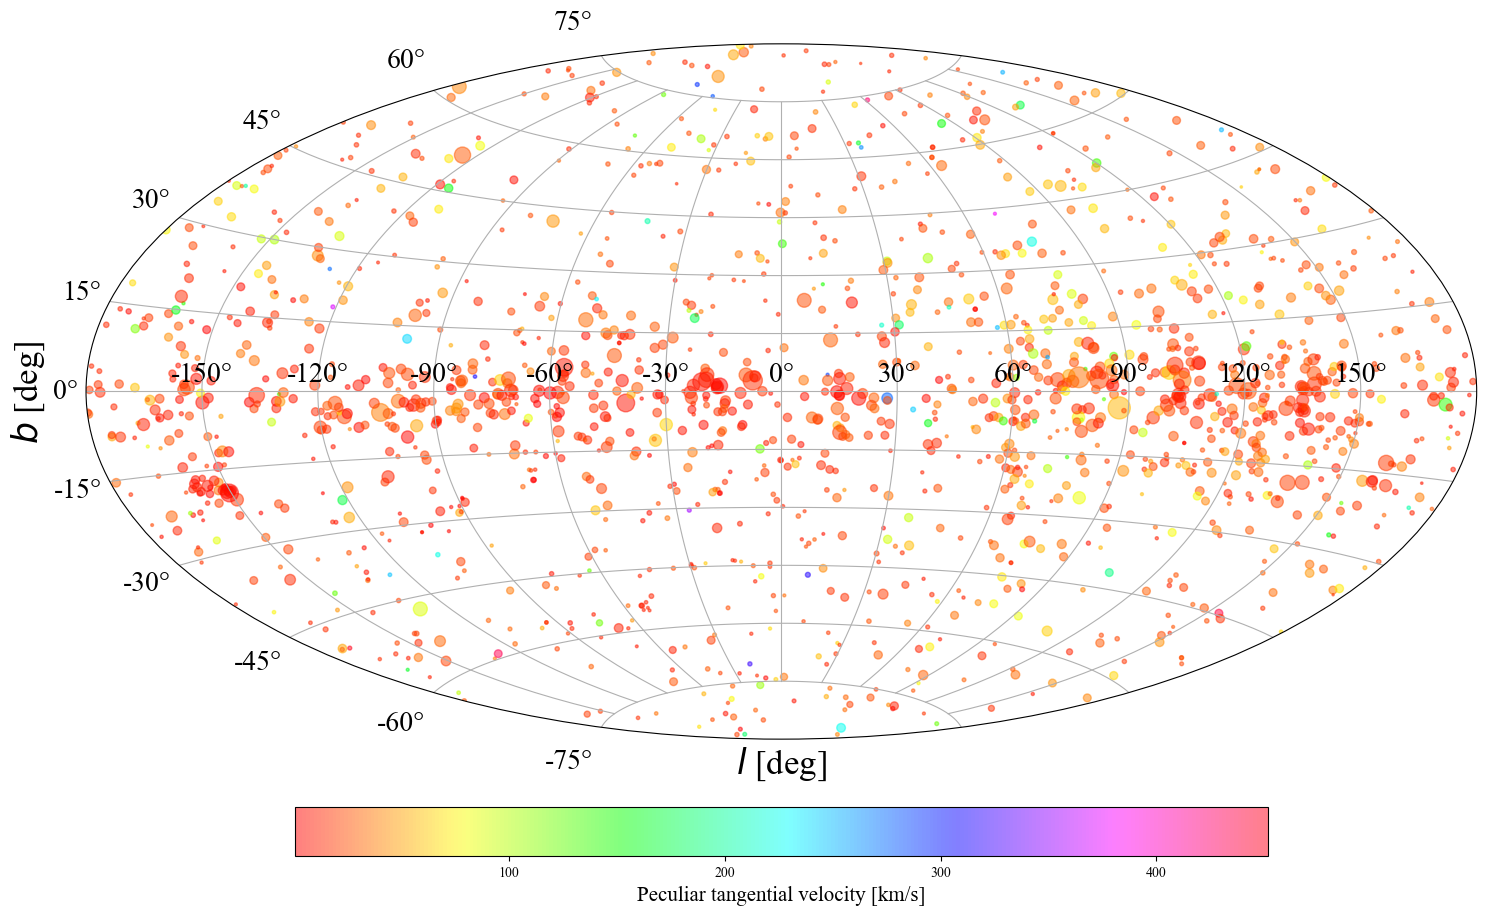
\includegraphics[width=1\textwidth]{aitoff}
                    \caption{Aitoffova projekce}
                    \label{fig:aitoff}
                \end{sidewaysfigure}
                \begin{sidewaysfigure}
                    \centering
                    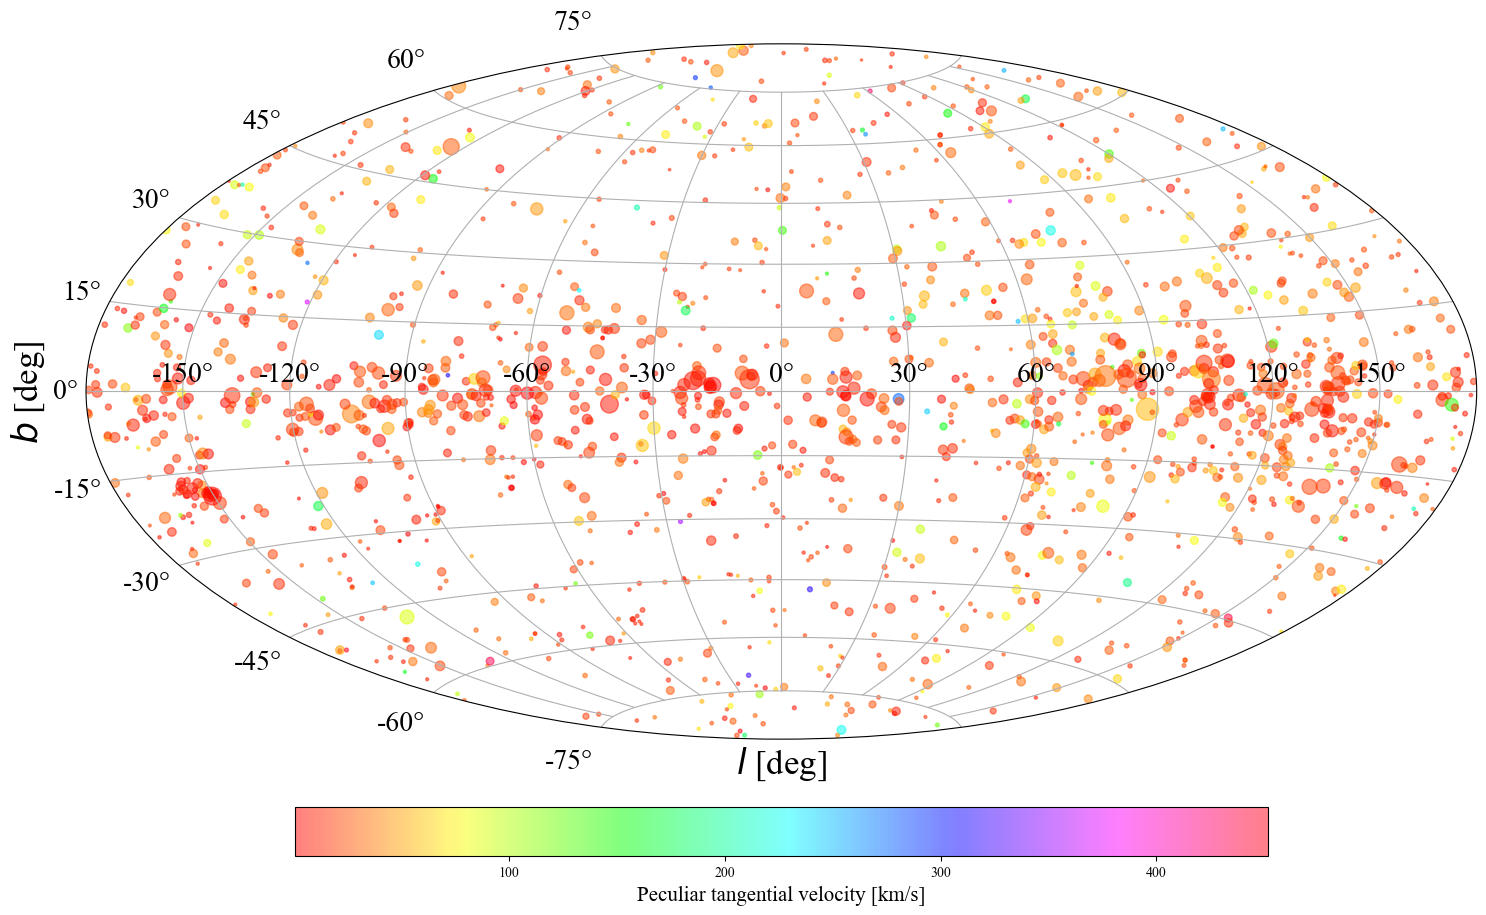
\includegraphics[width=1\textwidth]{hammer}
                    \caption{Hammerova projekce}
                    \label{fig:hammer}
                \end{sidewaysfigure}
                \begin{sidewaysfigure}
                    \centering
                    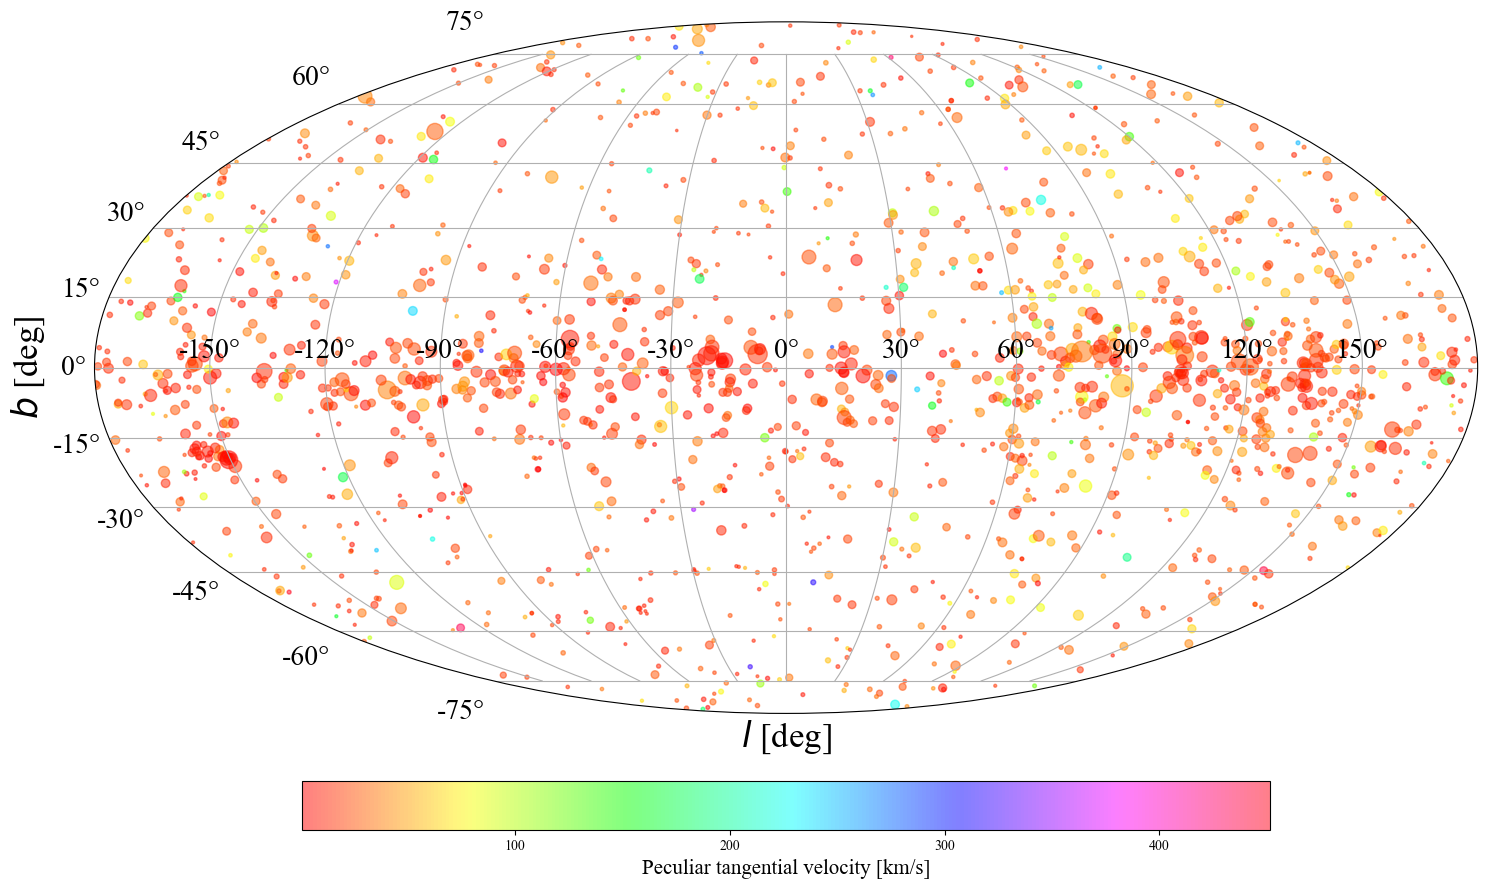
\includegraphics[width=1\textwidth]{mollweide}
                    \caption{Mollweideova projekce}
                    \label{fig:mollweide}
                \end{sidewaysfigure}
                \begin{sidewaysfigure}
                    \centering
                    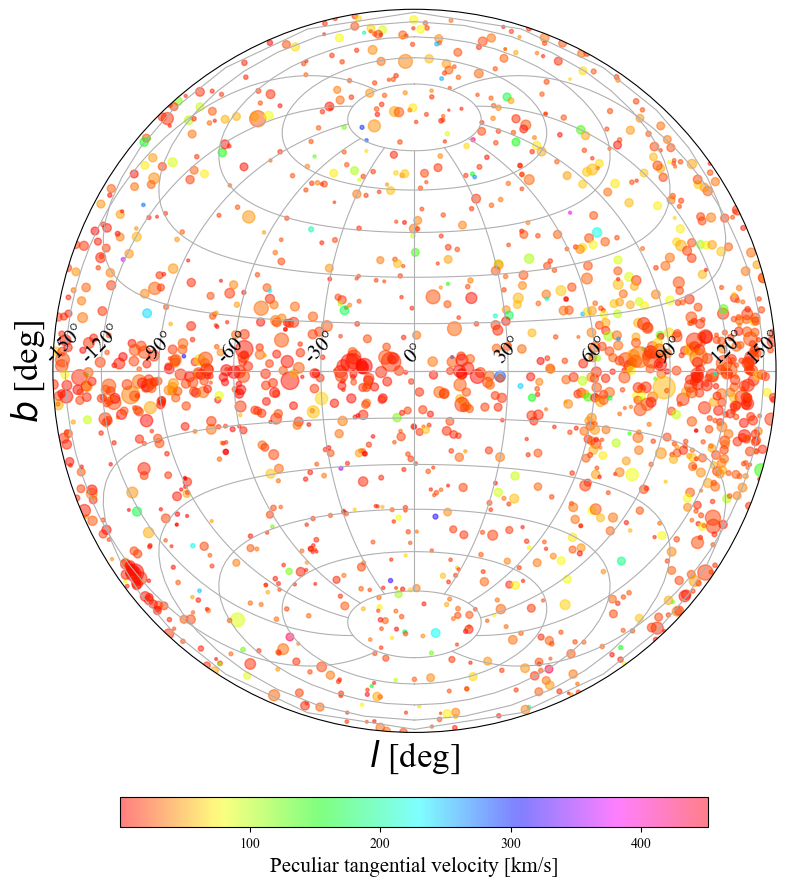
\includegraphics[width=0.7\textwidth]{lambert}
                    \caption{Lambertova projekce}
                    \label{fig:lambert}
                \end{sidewaysfigure}
\end{document}